\textbf{3. (Abstract game).}
Consider the following game:
\[
\begin{array}{c|ccccc}
 & t_1 & t_2 & t_3 & t_4 & t_5\\
\hline
s_1 & (2,0) & (5,3) & (2,4) & (6,1) & (3,2)\\
s_2 & (3,1) & (0,6) & (0,5) & (3,2) & (0,3)\\
s_3 & (4,6) & (1,3) & (2,1) & (5,4) & (1,3)\\
s_4 & (2,7) & (4,2) & (1,4) & (5,8) & (4,5)
\end{array}
\]
where the row player chooses \(s_1,s_2,s_3,s_4\) and the column player chooses \(t_1,t_2,t_3,t_4,t_5\).

\begin{enumerate}
\item[(a)]
By eliminating strictly dominated strategies reduce the game to the form \(2\times N\).
Specify which strategy is dominated by which one.
Note that a strategy may be dominated not only by a particular strategy but also by a mixture of strategies.
Any further eliminations must be impossible in the remaining game.

\item[(b)]
Find all pure and mixed equilibriums in the remaining \(2\times N\) game.
\end{enumerate}

\textbf{Solution.}

\textbf{(a) Elimination of strictly dominated strategies.}

\textbf{Step 1: eliminate \(s_2\).}
Compare the row-player payoffs of \(s_2\) and \(s_3\):
\[
(3,0,0,3,0) \quad \text{vs.} \quad (4,1,2,5,1)
\]
Since
\[
4>3,\quad 1>0,\quad 2>0,\quad 5>3,\quad 1>0,
\]
strategy \(s_3\) strictly dominates \(s_2\). Hence \(s_2\) is eliminated.

The reduced game is
\[
\begin{array}{c|ccccc}
 & t_1 & t_2 & t_3 & t_4 & t_5\\
\hline
s_1 & (2,0) & (5,3) & (2,4) & (6,1) & (3,2)\\
s_3 & (4,6) & (1,3) & (2,1) & (5,4) & (1,3)\\
s_4 & (2,7) & (4,2) & (1,4) & (5,8) & (4,5)
\end{array}
\]

\textbf{Step 2: eliminate \(t_5\).}

We want to show that column \(t_5\) is strictly dominated by a mixture of other columns.
Let the mixture of columns \(t_1, t_2, t_3, t_4\) have weights
\[
\alpha, \beta, \gamma, \delta \ge 0,
\qquad
\alpha + \beta + \gamma + \delta = 1
\]

Now calculate the expected payoffs of the mixture.

We only need to check the remaining rows \(s_1, s_3, s_4\).
The column player's expected payoffs are:

\begin{itemize}
\item Against \(s_1\):
\[
0\alpha + 3\beta + 4\gamma + 1\delta
\]

\item Against \(s_3\):
\[
6\alpha + 3\beta + 1\gamma + 4\delta
\]

\item Against \(s_4\):
\[
7\alpha + 2\beta + 4\gamma + 8\delta
\]
\end{itemize}

Compare with \(t_5\).

Column \(t_5\) yields payoffs
\[
(2,3,5)
\]

To strictly dominate \(t_5\), the mixture must satisfy:
\[
3\beta + 4\gamma + \delta > 2,
\]
\[
6\alpha + 3\beta + \gamma + 4\delta > 3,
\]
\[
7\alpha + 2\beta + 4\gamma + 8\delta > 5,
\]
together with
\[
\alpha + \beta + \gamma + \delta = 1,
\qquad
\alpha, \beta, \gamma, \delta \ge 0
\]

Thus we obtain a system of linear inequalities. Any solution gives a valid dominating mixture.

\textbf{Identify strong columns.}

Compare each column to \(t_5 = (2,3,5)\):

\begin{itemize}
\item For \(s_1\): need \(>2\), good columns are \(t_2 = 3\), \(t_3 = 4\)
\item For \(s_3\): need \(>3\), good columns are \(t_1 = 6\), \(t_4 = 4\)
\item For \(s_4\): need \(>5\), good columns are \(t_1 = 7\), \(t_4 = 8\)
\end{itemize}

Hence we try a mixture of \(t_2, t_3, t_4\):

\[
\frac13 t_2+\frac16 t_3+\frac12 t_4
\]
Its column-player payoffs against \(s_1,s_3,s_4\) are
\[
\left(\frac13\cdot 3+\frac16\cdot 4+\frac12\cdot 1,\;
\frac13\cdot 3+\frac16\cdot 1+\frac12\cdot 4,\;
\frac13\cdot 2+\frac16\cdot 4+\frac12\cdot 8\right)
=
\left(\frac{13}{6},\frac{19}{6},\frac{16}{3}\right)
\]
For \(t_5\), the column-player payoffs are
\[
(2,3,5)
\]
Since
\[
\frac{13}{6}>2,\qquad \frac{19}{6}>3,\qquad \frac{16}{3}>5,
\]
strategy \(t_5\) is strictly dominated by the mixture
\[
\frac13 t_2+\frac16 t_3+\frac12 t_4
\]
Hence \(t_5\) is eliminated.

The reduced game is now
\[
\begin{array}{c|cccc}
 & t_1 & t_2 & t_3 & t_4\\
\hline
s_1 & (2,0) & (5,3) & (2,4) & (6,1)\\
s_3 & (4,6) & (1,3) & (2,1) & (5,4)\\
s_4 & (2,7) & (4,2) & (1,4) & (5,8)
\end{array}
\]

\textbf{Step 3: eliminate \(s_4\).}
Consider the mixture
\[
\frac56 s_1+\frac16 s_3
\]
Its row-player payoffs against \(t_1,t_2,t_3,t_4\) are
\[
\left(\frac56\cdot 2+\frac16\cdot 4,\;
\frac56\cdot 5+\frac16\cdot 1,\;
\frac56\cdot 2+\frac16\cdot 2,\;
\frac56\cdot 6+\frac16\cdot 5\right)
=
\left(\frac73,\frac{13}{3},2,\frac{35}{6}\right)
\]
For \(s_4\), the row-player payoffs are
\[
(2,4,1,5)
\]
Since
\[
\frac73>2,\qquad \frac{13}{3}>4,\qquad 2>1,\qquad \frac{35}{6}>5,
\]
strategy \(s_4\) is strictly dominated by the mixture
\[
\frac56 s_1+\frac16 s_3
\]
Hence \(s_4\) is eliminated.

The reduced game is now
\[
\begin{array}{c|cccc}
 & t_1 & t_2 & t_3 & t_4\\
\hline
s_1 & (2,0) & (5,3) & (2,4) & (6,1)\\
s_3 & (4,6) & (1,3) & (2,1) & (5,4)
\end{array}
\]

\textbf{Step 4: eliminate \(t_4\).}
Consider the mixture
\[
\frac23 t_1+\frac13 t_3
\]
Its column-player payoffs against \(s_1,s_3\) are
\[
\left(\frac23\cdot 0+\frac13\cdot 4,\;
\frac23\cdot 6+\frac13\cdot 1\right)
=
\left(\frac43,\frac{13}{3}\right)
\]
For \(t_4\), the column-player payoffs are
\[
(1,4)
\]
Since
\[
\frac43>1,\qquad \frac{13}{3}>4,
\]
strategy \(t_4\) is strictly dominated by the mixture
\[
\frac23 t_1+\frac13 t_3
\]
Hence \(t_4\) is eliminated.

We arrive at the \(2\times 3\) game
\[
\boxed{
\begin{array}{c|ccc}
 & t_1 & t_2 & t_3\\
\hline
s_1 & (2,0) & (5,3) & (2,4)\\
s_3 & (4,6) & (1,3) & (2,1)
\end{array}}
\]

\textbf{No further eliminations are possible.}
For the row player, neither \(s_1\) nor \(s_3\) strictly dominates the other:
\[
2<4 \text{ at } t_1,\qquad 5>1 \text{ at } t_2
\]
For the column player, none of \(t_1,t_2,t_3\) is strictly dominated in the remaining game:
\begin{itemize}
\item \(t_1\) gives the highest payoff against \(s_3\),
\item \(t_3\) gives the highest payoff against \(s_1\),
\item \(t_2\) is not dominated since it will be a best response for some mixed strategy of the row player (see part (b)).
\end{itemize}

\textbf{(b) Pure and mixed Nash equilibriums in the remaining \(2\times 3\) game.}

We now analyze
\[
\begin{array}{c|ccc}
 & t_1 & t_2 & t_3\\
\hline
s_1 & (2,0) & (5,3) & (2,4)\\
s_3 & (4,6) & (1,3) & (2,1)
\end{array}
\]

\textbf{Pure Nash equilibriums.}

\textbf{Row player's best responses.}
\begin{itemize}
\item Against \(t_1\): \(2<4\), so the best response is \(s_3\).
\item Against \(t_2\): \(5>1\), so the best response is \(s_1\).
\item Against \(t_3\): \(2=2\), so both \(s_1\) and \(s_3\) are best responses.
\end{itemize}

\textbf{Column player's best responses.}
\begin{itemize}
\item Against \(s_1\): compare \(0,3,4\), so the best response is \(t_3\).
\item Against \(s_3\): compare \(6,3,1\), so the best response is \(t_1\).
\end{itemize}

Therefore the pure Nash equilibriums are
\[
\boxed{(s_3,t_1)\quad \text{and}\quad (s_1,t_3).}
\]

\textbf{Mixed Nash equilibriums.}

Let the row player choose \(s_1\) with probability \(p\), and \(s_3\) with probability \(1-p\).

Then the column player's expected payoffs are
\[
u_C(t_1)=0\cdot p+6(1-p)=6-6p,
\]
\[
u_C(t_2)=3,
\]
\[
u_C(t_3)=4p+1(1-p)=1+3p
\]

\textbf{Best responses of the column player.}
We compare:
\[
u_C(t_1)=u_C(t_2) \iff 6-6p=3 \iff p=\frac12,
\]
\[
u_C(t_2)=u_C(t_3) \iff 3=1+3p \iff p=\frac23
\]
Hence:
\begin{itemize}
\item if \(p<\frac12\), the unique best response is \(t_1\),
\item if \(p=\frac12\), the best responses are \(t_1,t_2\),
\item if \(\frac12<p<\frac23\), the unique best response is \(t_2\),
\item if \(p=\frac23\), the best responses are \(t_2,t_3\),
\item if \(p>\frac23\), the unique best response is \(t_3\).
\end{itemize}

\textbf{A fully mixed row player.}
Let the column player choose \(t_1,t_2,t_3\) with probabilities \(x,y,z\), where
\[
x+y+z=1
\]
The row player's expected payoffs are
\[
u_R(s_1)=2x+5y+2z,
\]
\[
u_R(s_3)=4x+y+2z
\]
For the row player to mix, we need indifference:
\[
2x+5y+2z=4x+y+2z
\]
which simplifies to
\[
4y=2x \iff x=2y. \tag{1}
\]

\textbf{Mixed equilibrium with support \(\{t_1,t_2\}\).}
At \(p=\frac12\), the column player's best responses are \(t_1,t_2\). So set \(z=0\). Then from
\[
x+y=1,\qquad x=2y,
\]
we obtain
\[
y=\frac13,\qquad x=\frac23
\]
Thus one mixed Nash equilibrium is
\[
\left(\frac12 s_1+\frac12 s_3,\ \frac23 t_1+\frac13 t_2\right)
\]

\textbf{Nash equilibriums in which the column player chooses \(t_3\).}
If the column player plays \(t_3\) purely, then the row player's payoffs are
\[
u_R(s_1)=2,\qquad u_R(s_3)=2,
\]
so any mixture of \(s_1\) and \(s_3\) is a best response.

For \(t_3\) to be a best response for the column player, we need
\[
u_C(t_3)\ge u_C(t_1),\qquad u_C(t_3)\ge u_C(t_2),
\]
that is,
\[
1+3p \ge 6-6p,\qquad 1+3p \ge 3
\]
\[
9p\ge 5 \iff p\ge \frac{5}{9},
\qquad
3p\ge 2 \iff p\ge \frac23
\]
So the condition is
\[
p\ge \frac23
\]

\begin{center}
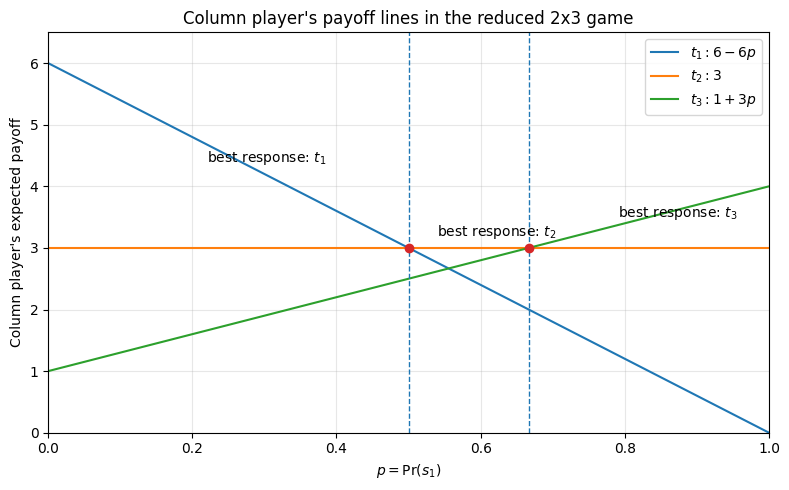
\includegraphics[width=1\linewidth]{problem_3_chart.png}
\end{center}

At \(p = \frac{1}{2}\) and \(p = \frac{2}{3}\), the column player is indifferent between two strategies.
Therefore, for every
\[
p\in\left[\frac23,1\right],
\]
the profile
\[
\left(p\,s_1+(1-p)\,s_3,\ t_3\right)
\]
is a Nash equilibrium.

\textbf{Final answer}

After elimination of strictly dominated strategies, the game reduces to
\[
\begin{array}{c|ccc}
 & t_1 & t_2 & t_3\\
\hline
s_1 & (2,0) & (5,3) & (2,4)\\
s_3 & (4,6) & (1,3) & (2,1)
\end{array}
\]

The pure Nash equilibriums in this remaining game are
\[
(s_3,t_1)\quad \text{and}\quad (s_1,t_3)
\]

The mixed Nash equilibriums are:
\[
\left(\frac12 s_1+\frac12 s_3,\ \frac23 t_1+\frac13 t_2\right)
\]
and the family
\[
\left(p\,s_1+(1-p)\,s_3,\ t_3\right),\qquad p\in\left[\frac23,1\right]
\]
